\subsection{可度量化拓扑群}

命题 1. 拓扑群 G 的左一致结构与右一致结构都可度量化，当且仅当 G 是豪斯多夫的且 G 的单位元 e 具有可数的基本邻域系。

该条件显然是必要的。反之，设它成立，令 \((\mathbf{V}_{n})\) 是 e 的一个基本邻域系；若以 \(U_{n}\) 表示诸对 \((x, y) \in \mathbf{G} \times \mathbf{G}\) 中满足 \(x^{-1}y \in V_{n}\) 者所成的集，则诸 \(U_{n}\) 构成 G 的左一致结构的一个可数围域基本系；由于此一致结构是豪斯多夫的，由 §2，第 4 号，定理 1 推出它是可度量化的。对 G 的右一致结构同理。

若拓扑群 G 的拓扑可度量化，则称 G 是可度量化的。于是命题 1 表明它的两个一致结构都是可度量化的。

借助下述概念，这一结果可以加强：

定义 1. 群 G（乘法记写）上的度量 d 称为左不变的（相应地，右不变的），如果我们有

\[
d (z x, z y) = d (x, y) \quad [ \text { resp. } d (x z, y z) = d (x, y) ]
\]

其中 \(x, y, z\) 取遍 \(\mathbf{G}\) 。

命题 2. 可度量化群 G 的左（相应地，右）一致结构可由 G 上的一个左不变（相应地，右不变）度量来定义。

设 e 的基本邻域系 \((\mathbf{V}_{n})\) 由对称邻域组成，使得 \(V_{n+1}^{3} \subset V_{n}\) 对每个 n 成立。~于是左一致结构的相应围域 \(U_{n}\) 是对称

的围域，且满足 \(\mathbf{U}_{n+1} \subset \mathbf{U}_n\) 。§1，第 4 号命题 2 的证明中所用的方法，使我们可以从围域序列 \((\mathbf{U}_n)\) 出发，构造出一个度量 \(d\) ，它定义在 \(\mathbf{G}\) 上且与 \(\mathbf{G}\) 的左一致结构相容；又因对每个 \(z \in \mathbf{G}\) ，映射 \((x, y) \to (zx, zy)\) 保持每个 \(\mathbf{U}_n\) 不变，由 \(d\) 的定义可知它是左不变度量。此方法对右一致结构同样适用。

注意，若 G 的两个一致结构不同，则度量 d 不是右不变的，因而一般地 \(d(x^{-1}, y^{-1}) \neq d(x, y)\) 。

特别地，若 G 是可度量化交换群，则它的一致结构由一个不变度量 d 定义；若 G 用加法记写，我们有

\[
d (x, y) = d (\mathrm{o}, y - x) = d (\mathrm{o}, x - y).
\]

我们常以 \(|x|\) （或 \(||x||\) ）表示 \(d(0, x)\) ；这时

\[
d (x, y) = | x - y |.
\]

函数 \(|x|\) 满足下列三个条件：

\begin{enumerate}
\def\labelenumi{\alph{enumi})}
\item
  \(|-x| = |x|\) 对一切 \(x \in G\) 成立。
\item
  \(|x + y| \leqslant |x| + |y|\) 对一切 \(x \in G\) 与一切 \(y \in G\) 成立。
\item
  \(|x| = 0\) 当且仅当 \(x = 0\) 。
\end{enumerate}

反之：

命题 3. 设 G 是用加法记写的交换群，\(x \to |x|\) 是满足上述条件 a)、b)、c) 的一个映射 \(\mathbf{G} \to \mathbf{R}_+\) 。则函数 \(d(x, y) = |x - y|\) 是 G 上的不变度量；它在 G 上定义的拓扑 C 与 G 的群结构相容，且由 d 定义的一致结构与赋有拓扑 C 的 G 所成拓扑群的一致结构相同。

函数 \(d(x, y)\) 是 \(G\) 上的度量，因为关系 \(d(x, y) = 0\) 等价于 \(x = y\) （由 \(c\) ）；而有 \(d(x, y) = d(y, x)\) （由 \(a\) ）；并且

\[
d (x, y) = | (x - z) + (z - y) | \leqslant | x - z | + | z - y | = d (x, z) + d (z, y)
\]

这是由 \(b\) ) 得到的。此外，\(d\) 是不变的，因为 \((x + z) - (y + z) = x - y\) 。对每个实数 \(\alpha > 0\) ，令 \(V_{\alpha}\) 为全体 \(x \in G\) 中满足 \(|x| < \alpha\) 者所成的集；则诸 \(V_{\alpha}\) 构成一个基本邻域系 \(\mathfrak{S}\) ，即 \(o\) 关于拓扑 \(\mathfrak{C}\) 的基本邻域系；又因 \(d\) 不变，\(a + \mathfrak{S}\) 是 \(a\) 的一个基本邻域系（关于拓扑 \(\mathfrak{C}\) ；这里 \(a \in G\) 任意）。由 \(a\) ，诸 \(V_{\alpha}\) 是对称的；由 \(b\) ，有 \(V_{\alpha} + V_{\alpha} \subset V_{2\alpha}\) ；因而拓扑 \(\mathfrak{C}\) 与 \(G\) 的群结构相容（第 III 章，§ 1，第 2 号）。命题的最后一部分立即可得。

条件 \(a), b)\) 与 \(c)\) 等价于 \(c)\) 连同条件

\[
| x - y | \leqslant | x | + | y |.\tag{\(b^{\prime}\)}
\]

因为 \(a)\) 与 \(b)\) 显然蕴含 \(b')\) ；反之，取 \(x = 0\) 代入 \(b')\) 并利用 \(c)\) ，得 \(|-y| \leqslant |y|\) ；把 \(y\) 换成 \(-y\) 便得 \(|-y| = |y|\) ，此即 \(a)\) ；再把 \(y\) 换成 \(-y\) 代入 \(b')\) 即得 \(b)\) 。

命题 4. 若 G 是可度量化群，则 G 的每个豪斯多夫商群 G/H 都可度量化。若 G 还是完备的，则 G/H 是完备的 (*)。

命题的第一部分是如下事实的推论：G/H 的单位元在 G/H 中具有可数的基本邻域系；因为若 \((\mathbf{V}_{n})\) 是 e 在 G 中的基本邻域系，则 \(\dot{V}_{n}\) （诸集 \(V_{n}\) 在 G/H 中的典范像）构成 G/H 的单位元的基本邻域系（第 III 章，§ 2，第 6 号，命题 17）。

要证明当 G 完备时 G/H 也完备，由 § 2，第 6 号，命题 9，只需证明每个柯西序列 \((\dot{x}_{n})\) （关于 G/H 的左一致结构）都收敛。必要时可代之以 \((\dot{x}_{n})\) 的子序列，从而可设对每对满足 \(p \geqslant n\) 且 \(q \geqslant n\) 的指标 p、q，有 \(\dot{x}_{p}^{-1}\dot{x}_{q} \in \dot{V}_{n}\) ；这表示对每对点 \(y \in \dot{x}_{p}, z \in \dot{x}_{q}\) ，有 \(y^{-1}z \in HV_{n} = V_{n}H\) ；因而对每个 \(y \in \dot{x}_{p}\) ，\(\dot{x}_{q}\) 与 y 的邻域 \(yV_{n}\) 之交非空。现设序列 \((V_{n})\) 已选得使 \(V_{n+1}^{2} \subset V_{n}\) ，并归纳地定义 G 中点的序列 \((x_{n})\) ，使得 \(x_{n} \in \dot{x}_{n}\) 且 \(x_{n+1} \in x_{n}V_{n}\) ；由前所述这是可能的。于是由归纳法推出，对每个 p \textgreater{} 0 有 \(x_{n+p} \in x_{n}V_{n}V_{n+1} \ldots V_{n+p-1} \subset x_{n}V_{n-1}\) 。因此序列 \((x_{n})\) 是 G 中的柯西序列，故收敛于一点 a；并且立即得出，a 在 G/H 中的典范像 \(\dot{a}\) 是序列 \((\dot{x}_{n})\) 的极限。

推论 1. 设 G 是完备可度量化群，\(G_{0}\) 是 G 的稠密子群，\(H_{0}\) 是 \(G_{0}\) 的闭正规子群。若 H 是 \(H_{0}\) 在 G 中的闭包，则商群 \(G_{0}/H_{0}\) 的完备化同构于 G/H。

H 是 G 的正规子群（第 III 章，§ 2，第 3 号，命题 8），且命题 4 表明 G/H 是完备的。又若 \(\varphi\) 是 G 到 G/H 上的典范映射，则显然 \(\varphi(G_0)\) 在 G/H 中稠密。因此结论由第 III 章，§ 2，第 7 号，命题 21 得出。

设 \(G, G'\) 是两个豪斯多夫交换拓扑群，\(\hat{G}, \hat{G}'\) 是它们各自的完备化。我们回忆（第 III 章，§ 3，第 3 号，命题 5）：若 \(u\) 是 \(G\) 到 \(G'\) 中的连续同态，则 \(u\) 一致连续，且可唯一扩张为 \(\hat{G}\) 到 \(\hat{G}'\) 中的连续同态 \(\hat{u}\) ，在以下

本小节的其余部分中即用此记号。图表

\pandocbounded{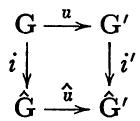
\includegraphics[keepaspectratio]{images/part001_945be03d.jpg}}

（其中 \(i\) ， \(i'\) 是典范单射）是交换的。若 \(v\) 是 \(\mathbf{G}'\) 到豪斯多夫交换拓扑群 \(\mathbf{G}''\) 中的连续同态，且 \(w = v \circ u\) ，则立即得出 \(\hat{w} = \hat{v} \circ \hat{u}\) 。

设 H 是 G 的闭子群，令 E = G/H。设 \(j: H \to G\) 与 \(p: G \to E\) 是典范映射。设 \(\overline{H}\) 是 H 在 \(\hat{G}\) 中的闭包；\(\overline{H}\) 是完备群，我们把它与 H 的完备化 \(\hat{H}\) 等同。j 的连续延拓 \(\hat{j}\) （到 \(\hat{H}\) 上）显然是 \(\hat{H}\) 到 \(\hat{G}\) 中的典范单射。

以下设 G 是可度量化的。于是 E = G/H 到 \(\hat{G}/\hat{H}\) 中的典范映射是 E 到完备群 \(\hat{G}/\hat{H}\) 的一个稠密子群上的拓扑同构（推论 1），从而我们可把 \(\hat{G}/\hat{H}\) 与 \(\hat{E}\) 等同，并把 p 的连续延拓 \(\hat{p}\) （到 \(\hat{G}\) 上）与 \(\hat{G}\) 到 \(\hat{G}/\hat{H}\) 上的典范映射等同。

推论 2. 设 G，G‘ 是两个可度量化交换拓扑群；u: G → G’ 是严格态射，其核为 N、像为 P。则 \(\hat{u} : \hat{G} \rightarrow \hat{G}'\) 是严格态射，其核为 \(\hat{N}\) 、像为 \(\hat{P}\) 。

设 \(u = j \circ v \circ p\) 是 \(u\) 的典范分解，其中 \(v\) 是拓扑群 \(G/N\) 到拓扑群 \(u(G) = P\) 上的同构。我们有 \(\hat{u} = \hat{j} \circ \hat{v} \circ \hat{p}\) ，并且已经看到 \(\hat{p}\) 是 \(\hat{G}\) 到 \(\hat{G}/\hat{N}\) 上的典范映射，而 \(\hat{j}\) 是 \(\hat{P}\) 到 \(\hat{G}'\) 中的典范映射。另一方面，\(\hat{v}\) 是 \(\hat{G}/\hat{N}\) 到 \(\hat{P}\) 上的同构（第 III 章，§ 3，第 4 号，命题 5），由此即得结论。

推论 3. 设 \(\mathbf{G}, \mathbf{G}'\) ， \(\mathbf{G}''\) 是三个可度量化交换拓扑群，\(u: \mathbf{G} \to \mathbf{G}'\) 与 \(v: \mathbf{G}' \to \mathbf{G}''\) 是两个严格态射，使得序列 \(\mathbf{G} \xrightarrow{u} \mathbf{G}' \xrightarrow{v} \mathbf{G}''\) 是正合的{[}即 \(u(\mathbf{G}) = \overline{v}^{1}(\mathbf{o})\) {]}。则序列 \(\hat{\mathbf{G}} \xrightarrow{\hat{u}} \hat{\mathbf{G}}' \xrightarrow{\hat{v}} \hat{\mathbf{G}}''\) 是正合的。

因为若令 \(\mathrm{N} = u(\mathrm{G}) = \overline{v}^{1}(\mathrm{o})\) ，则由推论 2，\(\hat{N}\) 既是 \(\hat{u}\) 的像又是 \(\hat{v}\) 的核。

注。1) 设 G 是非豪斯多夫拓扑群，但与之相伴的豪斯多夫群可度量化；等价地，G 的单位元在 G 中具有可数的基本邻域系。命题 4 的证明可不加修改地用于这一情形（H 为 G 的任意正规子群），它表明与 G/H 相伴的豪斯多夫群可度量化，并且只要 G 完备，G/H 就是完备群（一般不是豪斯多夫的）。

\begin{enumerate}
\def\labelenumi{\arabic{enumi})}
\setcounter{enumi}{1}
\tightlist
\item
  设 \(d\) 是定义可度量化群 G 的拓扑的左不变度量，H 是 G 的闭正规子群。若 \(\dot{x}\) 与 \(\dot{y}\) 是 G/H 的任意两点，考虑距离 \(d(\dot{x},\dot{y})\) ，即 G 中两个闭子集 \(\dot{x},\dot{y}\) 之间的距离（§ 2，第 2 号）；我们将看到，这个函数是 G/H 上的左不变度量，并且定义这个商群的拓扑。
\end{enumerate}

首先注意，若 \(x \in \dot{x}\) 且 \(y \in \dot{y}\) ，则有 \(d(\dot{x}, \dot{y}) = d(x, \mathrm{H}y)\) ；因为 \(d(x, \mathrm{H}y) = \inf_{h \in \mathbf{H}} d(x, h y)\) ，从而 \(d(h' x, \mathrm{H} y) = d(x, \mathrm{H} y)\) 对一切 \(h' \in \mathrm{H}\) 成立，因为 \(d\) 是左不变的；这就证明了断言（§ 2，第 2 号）。于是对每个 \(\dot{z} \in \mathrm{G} / \mathrm{H}\) 有{[}§ 2，第 2 号，公式 (2){]}

\[
\left| d (\dot {x}, \dot {z}) - d (\dot {y}, \dot {z}) \right| = \left| d (x, \dot {z}) - d (y, \dot {z}) \right| \leqslant d (x, y);
\]

又因这个不等式对一切 \(x \in \dot{x}\) 与一切 \(y \in \dot{y}\) 成立，我们有 \(|d(\dot{x}, \dot{z}) - d(\dot{y}, \dot{z})| \leqslant d(\dot{x}, \dot{y})\) ，这表明 \(d(\dot{x}, \dot{y})\) 是 G/H 上的度量。此外，对任意 \(z \in \dot{z}\) ，我们有

\[
d (\dot {z} \dot {x}, \dot {z} \dot {y}) = \inf _ {h \in \mathbf {H}} d (z x, h z y)
\]

这是由上面的式子得到的；但由于 \(hzy = z(z^{-1}hz)y\) ，并且 \(z^{-1}hz\) 随 \(h\) 取遍 H 而取遍 H（H 是正规的），\(d(x,y)\) 的左不变性表明有 \(d(zx, \mathrm{Hz}) = d(x, \mathrm{Hy}) = d(\dot{x}, \dot{y})\) 。最后，若 V 是 G 中 \(e\) 的由 \(d(e, x) < \alpha\) 定义的邻域，则 V 在 G/H 中的像 V 就是由 \(d(\dot{e}, \dot{x}) < \alpha\) 定义的集；这就完成了证明。

